\documentclass[12pt]{report}
\usepackage[spanish]{babel}
\usepackage[utf8]{inputenc}
\usepackage{amsmath}
\usepackage{amssymb}
\usepackage{amsthm}
\usepackage{graphics}
\usepackage{subfigure}
\usepackage{lipsum}
\usepackage{array}
\usepackage{multicol}
\usepackage{enumerate}
\usepackage[framemethod=TikZ]{mdframed}
\usepackage[a4paper, margin = 1.5cm]{geometry}
\usepackage{enumitem}
\usepackage{tikz}
\usepackage{pgffor}
\usepackage{ifthen}
\usepackage{bbm}

\usetikzlibrary{shapes.multipart}

\newcounter{it}
\newcommand*\watermarktext[1]{\begin{tabular}{c}
    \setcounter{it}{1}%
    \whiledo{\theit<100}{%
    \foreach \col in {0,...,15}{#1\ \ } \\ \\ \\
    \stepcounter{it}%
    }
    \end{tabular}
    }

\AddToHook{shipout/foreground}{
    \begin{tikzpicture}[remember picture,overlay, every text node part/.style={align=center}]
        \node[rectangle,black,rotate=30,scale=2,opacity=0.04] at (current page.center) {\watermarktext{Cristo Daniel Alvarado ESFM\quad}}; 
  \end{tikzpicture}
}
%En esta parte se hacen redefiniciones de algunos comandos para que resulte agradable el verlos%

\renewcommand{\theenumii}{\roman{enumii}}

\def\proof{\paragraph{Demostración:\\}}
\def\endproof{\hfill$\blacksquare$}

\def\sol{\paragraph{Solución:\\}}
\def\endsol{\hfill$\square$}

%En esta parte se definen los comandos a usar dentro del documento para enlistar%

\newtheoremstyle{largebreak}
  {}% use the default space above
  {}% use the default space below
  {\normalfont}% body font
  {}% indent (0pt)
  {\bfseries}% header font
  {}% punctuation
  {\newline}% break after header
  {}% header spec

\theoremstyle{largebreak}

\newmdtheoremenv[
    leftmargin=0em,
    rightmargin=0em,
    innertopmargin=0pt,
    innerbottommargin=5pt,
    hidealllines = true,
    roundcorner = 5pt,
    backgroundcolor = gray!60!red!30
]{exa}{Ejemplo}[section]

\newmdtheoremenv[
    leftmargin=0em,
    rightmargin=0em,
    innertopmargin=0pt,
    innerbottommargin=5pt,
    hidealllines = true,
    roundcorner = 5pt,
    backgroundcolor = gray!50!blue!30
]{obs}{Observación}[section]

\newmdtheoremenv[
    leftmargin=0em,
    rightmargin=0em,
    innertopmargin=0pt,
    innerbottommargin=5pt,
    rightline = false,
    leftline = false
]{theor}{Teorema}[section]

\newmdtheoremenv[
    leftmargin=0em,
    rightmargin=0em,
    innertopmargin=0pt,
    innerbottommargin=5pt,
    rightline = false,
    leftline = false
]{propo}{Proposición}[section]

\newmdtheoremenv[
    leftmargin=0em,
    rightmargin=0em,
    innertopmargin=0pt,
    innerbottommargin=5pt,
    rightline = false,
    leftline = false
]{cor}{Corolario}[section]

\newmdtheoremenv[
    leftmargin=0em,
    rightmargin=0em,
    innertopmargin=0pt,
    innerbottommargin=5pt,
    rightline = false,
    leftline = false
]{lema}{Lema}[section]

\newmdtheoremenv[
    leftmargin=0em,
    rightmargin=0em,
    innertopmargin=0pt,
    innerbottommargin=5pt,
    roundcorner=5pt,
    backgroundcolor = gray!30,
    hidealllines = true
]{mydef}{Definición}[section]

\newmdtheoremenv[
    leftmargin=0em,
    rightmargin=0em,
    innertopmargin=0pt,
    innerbottommargin=5pt,
    roundcorner=5pt
]{excer}{Ejercicio}[section]

%En esta parte se colocan comandos que definen la forma en la que se van a escribir ciertas funciones%

\newcommand\abs[1]{\ensuremath{\big|#1\big|}}
\newcommand\divides{\ensuremath{\bigm|}}
\newcommand\cf[3]{\ensuremath{#1:#2\rightarrow#3}}
\newcommand\contradiction{\ensuremath{\#_c}}
\newcommand{\Obj}[1]{\ensuremath{\textup{Obj}\left(#1\right)}}
\newcommand{\Hom}[3]{\ensuremath{\textup{Hom}_{#1}\left(#2,#3\right)}}

\newcommand{\Cat}[1]{\ensuremath{\textup{\textbf{#1}}}}
\newcommand{\Iso}[3]{\ensuremath{\textup{I}_{\textup{SO}_{#1}}\left(#2,#3\right)}}
\newcommand{\SO}[1]{\ensuremath{\textup{SO}\left(#1\right)}}
\newcommand{\Quo}[1]{\ensuremath{\textup{Quo}\left(#1 \right)}}
\newcommand{\bbm}[1]{\mathbbm{#1}}
\newcommand{\im}{\ensuremath{\textup{Im}}}
\newcommand{\coim}{\textup{Coim}}
    \newcommand{\coker}{\textup{Coker}}

%recuerda usar \clearpage para hacer un salto de página

\begin{document}
    \setlength{\parskip}{5pt} % Añade 5 puntos de espacio entre párrafos
    \setlength{\parindent}{12pt} % Pone la sangría como me gusta
    \title{Notas de Álgebra Moderna IV.
    
    Módulos.}
    \author{Cristo Daniel Alvarado}
    \maketitle

    \tableofcontents %Con este comando se genera el índice general del libro%

    %\setcounter{chapter}{3} %En esta parte lo que se hace es cambiar la enumeración del capítulo%

    \chapter{Módulos, Homomorfismos y Secuencias exactas}

    \section{Módulos y homomorfismos}

    Los módulos son una generalización de los grupos abelianos y lo enteros (los cuales son módulos sobre $\mathbb{Z}$).

    \begin{mydef}
        Sea $R$ un anillo no trivial. Decimos que $R$ es un \textbf{anillo de división}, si $R$ es unitario y para cada $a\in A$ existe $a^{-1}\in A$.

        Si $R$ es conmutativo, entonces $R$ es un \textbf{campo}.
    \end{mydef}

    \begin{mydef}
        Sea $R$ un anillo, un \textbf{$R$-módulo (izquierdo)} es un grupo abeilano $A$ junto con una función $\cf{\cdot}{R\times A}{A}$ (denotada simplemente por $(r,a)\mapsto ra$) tal que para todo $r,s\in R$ y para todo $a\in A$:
        \begin{enumerate}[label=\textit{(\arabic*)}]
            \item $r(a+b)=ra+rb$.
            \item $(r+s)a=ra+sa$.
            \item $r(sa)=(rs)a$.
        \end{enumerate}
        si $R$ además tiene elemento identidad $1_R$ y se cumple que
        \begin{enumerate}[label=\textit{(\arabic*)}]
            \setcounter{enumi}{3}
            \item $1_Ra=a$, para todo $a\in A$.
        \end{enumerate}
        entonces decimos que $A$ es un \textbf{$R$-módulo unitario (izquierdo)}. En caso de que $R$ sea un anillo de división, el módulo unitario $A$ será llamado \textbf{espacio vectorial (izquierdo)}.
    \end{mydef}

    De forma análoga podemos definir los $R$-módulos derechos, cambiando el orden en el que se hacen las operaciones. Sin embargo, a lo largo del texto solo trabajaremos con módulos izquierdos y todos los resultados que se prueben para esto, también se cumplirán para los derechos.
    
    \begin{excer}
        Sea $A$ un $R$-módulo izquierdo. Si $R$ es conmutativo, podemos hacer de $A$ un $R$-módulo derecho definiendo:
        \begin{equation*}
            ar = ra,\quad\forall a\in A\textup{ y }\forall r\in R
        \end{equation*}
    \end{excer}

    \begin{proof}
        Considere la función de $\cf{\cdot}{A\times R}{A}$ dada por:
        \begin{equation*}
            (a,r)\mapsto ar=ra,\quad\forall (a,r)\in A\times R
        \end{equation*}
        Afirmamos que esta función hace de $A$ un $R$-módulo derecho. En efecto, debemos verificar tres condiciones, sean $r,s\in R$ y $a,b\in A$:
        \begin{enumerate}[label=\textit{(\arabic*)}]
            \item Se tiene que:
            \begin{equation*}
                \begin{split}
                    (a+b)r&=r(a+b)\\
                    &=ra+rb\\
                    &=ar+br\\
                \end{split}
            \end{equation*}
            \item Se tiene que:
            \begin{equation*}
                \begin{split}
                    a(r+s)&=(r+s)a\\
                    &=ra+sa\\
                    &=ar+as\\
                \end{split}
            \end{equation*}
            \item Se tiene que:
            \begin{equation*}
                \begin{split}
                    (as)r&=r(as)\\
                    &=r(sa)\\
                    &=(rs)a\textup{, como $R$ es conmutativo:} \\
                    &=(sr)a\\
                    &=a(sr)\\
                \end{split}
            \end{equation*}
        \end{enumerate}
        por los tres incisos anteriores se sigue que $A$ es un $R$-módulo derecho.
    \end{proof}

    \begin{obs}
        A menos que se especifique lo contrario, todo $R$-módulo $A$ sobre un anillo conmutativo $R$ será izquierdo y derecho haciendo:
        \begin{equation*}
            ra=ar,\quad\forall a\in A\textup{ y }\forall r\in R
        \end{equation*}
    \end{obs}

    \begin{obs}
        Denotaremos al elemento identidad de un $R$-módulo $A$ por $0_A$, y al elemento neutro de $R$ por $0_R$.
    \end{obs}

    \begin{propo}
        Sea $A$ un $R$-módulo, entonces:
        \begin{equation*}
            r0_A=0_A\quad\textup{y}\quad 0_Ra=0_A
        \end{equation*}
        para todo $r\in R$ y para todo $a\in A$.
    \end{propo}

    \begin{proof}
        Sea $r\in R$, se tiene que:
        \begin{equation*}
            r0_A=r(0_A+0_A)=r0_A+r0_A\Rightarrow r0_A=0_A
        \end{equation*}
        y, para todo $a\in A$:
        \begin{equation*}
            0_Ra=(0_R+0_R)a=0_Ra+0_Ra\Rightarrow 0_Ra=0_A
        \end{equation*}
    \end{proof}

    Por lo que, en lo que sigue del texto se denotará por 0 a $0_A,0_R$, $0\in\mathbb{Z}$ y al módulo trivial $\left\{0\right\}$.

    \begin{exa}
        Todo grupo abeliano $G$ es un $\mathbb{Z}$ módulo unitario izquierdo (en particular, puede ser derecho por ser abeliano), bajo la operación $(n,a)\mapsto na $, siendo $na$ la suma de $a$ consigo mismo $n$-veces.
    \end{exa}

    \begin{exa}
        Si $S$ es un anillo y $R$ es un subanillo, entonces $S$ es un $R$-módulo (pero no al revés, ya que puede que la operación se salga de $S$) con $ra$ siendo $r\in R$ y $a\in S$. En particular, los anillos:
        \begin{equation*}
            R[x_1,...,x_n]\quad\textup{y}\quad R[[x]]
        \end{equation*}
        son $R$-módulos, los cuáles son unitarios si $R$ posee identidad.
    \end{exa}

    \begin{exa}
        Sean $R$, $S$ anillos y $\cf{\varphi}{R}{S}$ un homomorfismo de anillos. Entonces todo $S$-módulo puede hacerse un $R$-módulo definiendo $rx$ (con $x\in A$) por $\varphi(r)x$, esto es:
        \begin{equation*}
            rx=\varphi(r)x
        \end{equation*}
        donde la operación de la derecha se toma en el $S$-módulo, $A$. En este caso se dice que la estructura de $R$-módulo de $A$ está dada por el \textbf{pullback a lo largo de $\varphi$}.
    \end{exa}

    \begin{mydef}
        Sean $A$ y $B$ módulos sobre un anillo $R$. Una función $\cf{f}{A}{B}$ es un \textbf{homomorfismo de $R$-módulos}, si para todo $a,b\in A$ y para todo $r\in R$ se tiene que:
        \begin{equation*}
            f(a+b)=f(a)+f(b)\quad\textup{y}\quad f(ra)=rf(a)
        \end{equation*}
        si $R$ es un anillo de división, entonces $f$ es llamada \textbf{transformación lineal}.
    \end{mydef}

    En el contexto actual, los homomorfismos de $R$-módulos serán simplemente llamados homomorfismos. Se adopta la misma terminología de monomorfismo, epimorfismo e isomorfismo. Se define también de forma análoga el \textbf{núcleo} o \textbf{kernel} de $f$ por:
    \begin{equation*}
        \ker(f)=\left\{a\in A\Big|f(a)=0 \right\}
    \end{equation*}
    con lo que se tienen los siguientes resultados (que provienen directamente de lo probado en anillos):

    \begin{theor}
        Sean $A$ y $B$ dos $R$-módulos y $\cf{f}{A}{B}$ un homomorfismo.
        \begin{enumerate}[label = \textit{(\alph*)}]
            \item $f$ es monomorfismo si y sólo si $\ker(f)=\left\{0 \right\}$.
            \item $f$ es isomorfismo si y sólo si existe un homomorfismo de $R$-módulos $\cf{g}{B}{A}$ tal que $g\circ f = \bbm{1}_A$ y $f\circ g=\bbm{1}_B$.
        \end{enumerate}
    \end{theor}

    \begin{exa}
        Todo homomorifsmo entre grupos abelianos es un homomorfismo de $\mathbb{Z}$-módulos.
    \end{exa}

    \begin{exa}
        Si $R$ es un anillo, la función de $R[x]$ en $R[x]$ dada por: $f(x)\mapsto xf(x)$ es un homomorfismo de $R$-módulos, pero no es un homomorfismo de anillos (no separa productos).
    \end{exa}

    \begin{obs}
        Para un anillo $R$ dado, la clase de todos los $R$-módulos forma una categoría concreta, denotada por $\mathcal{M}_R$ para los módulos derechos y ${}_R\mathcal{M}$ para los izquierdos.
    \end{obs}

    \begin{mydef}
        Sea $R$ un anillo, $A$ un $R$-módulo y $B\subseteq A$ un subconjunto no vacío. Se dice que $B$ es un \textbf{submódulo de $A$} si $B$ es un subgrupo aditivo de $A$ y, para todo $r\in R$ se tiene que:
        \begin{equation*}
            rb\in B,\quad\forall b\in B
        \end{equation*}
        un submódulo de un espacio vectorial es llamado \textbf{subespacio vectorial}.
    \end{mydef}

    \begin{obs}
        Todo submódulo es en sí mismo un módulo. Todo submódulo de un módulo unitario es también untario.
    \end{obs}

    \begin{exa}
        Si $\left\{B_i\Big|i\in I \right\}$ es una familia de submódulos de un módulo $A$, entonces $\bigcap_{ i\in I}B_i$ es un submódulo de $A$.
    \end{exa}

    \begin{mydef}
        Sea $A$ un $R$-módulo y $X\subseteq A$, entonces la intersección de todos los submódulos que contienen a $X$ es llamado el \textbf{submódulo generado por $X$}.
    \end{mydef}

    Si $X$ es finito y $X$ genera al módulo $B$, se dice que $B$ es \textbf{finitamente generado}. Si $X$ tiene un solo elemento, se dice que $B$ es un \textbf{módulo cíclico}.

    Si $\left\{B_i \right\}_{ i\in I}$ es una familia de submódulos de $A$, entonces el submódulo generado por $\bigcup_{ i\in I}B_i$ es llamado la \textbf{suma de los módulos $B_i$}. Si el conjunto $I$ es finito, esto se denota por:
    \begin{equation*}
        B_1+\cdots+B_n
    \end{equation*}

    \begin{theor}
        Sea $R$ un anillo, $A$ un $R$-módulo, $X\subseteq X$, $\left\{B_i \right\}_{ i\in I}$ una familia de submódulos de $A$ y $a\in A$. Tomemos $Ra=\left\{ra\Big|r\in R \right\}$.
        \begin{enumerate}[label = \textit{(\alph*)}]
            \item $Ra$ es un submódulo de $A$ y la función de $R$ en $Ra$ dada por $r\mapsto ra$ es un epimorfismo de $R$-módulos.
            \item El submódulo cíclico $C$ generado por $a$ es
            \begin{equation*}
                \left\{ra+na\Big|r\in R,n\in\mathbb{Z} \right\}
            \end{equation*}
            si $R$ tiene identidad y $C$ es unitario, entonces $C=Ra$.
            \item El submódulo $D$ generado por $X$ es:
            \begin{equation*}
                \left\{\sum_{ i=1}^s r_ia_i+\sum_{ j=1}^t n_jb_j\Big|s,t\in\mathbb{N}^*;a_i,b_j\in X;r_i\in R;n_j\in\mathbb{Z} \right\}
            \end{equation*}
            si $R$ tiene identidad y $A$ es unitario, entonces:
            \begin{equation*}
                D=RX=\left\{\sum_{ i=1}^s r_ia_r\Big|i\in\mathbb{N}^*;r_i\in R;a_i\in X \right\}
            \end{equation*}
            \item La suma de la familia $\left\{B_i\Big|i\in I \right\}$ consiste de todas las sumas finitas $b_1+\cdots+b_{ i_n}$ con $b_{ i_k}\in B_{ i_k}$ para todo $k=1,...,n$.
        \end{enumerate}
    \end{theor}

    \begin{proof}
        De \textit{(a)}: Veamos que $Ra$ es un $R$-módulo. Claramente $s(ra)$ está bien definida (sigue en $Ra$ ya que $A$ es un $R$-módulo). Veamos que:
        \begin{itemize}
            \item Sean $ra,sa\in Ra$, entonces:
            \begin{equation*}
                \begin{split}
                    t(ra+sa)&=t(ra)+t(sa)\\
                \end{split}
            \end{equation*}
            \item Sean $r,s\in R$ y $ta\in Ra$, entonces:
            \begin{equation*}
                \begin{split}
                    (r+s)(ta)&=((r+s)t)a\\
                    &=(rt+st)a\\
                    &=(rt)a+(st)a\\
                    &=r(ta)+s(ta)\\
                \end{split}
            \end{equation*}
            \item Sean $r,s\in R$ y $ta\in Ra$, entonces:
            \begin{equation*}
                \begin{split}
                    r(s(ta))&=r((st)a)\\
                    &=(r(st))a\\
                    &=((rs)t)a\\
                    &=(rs)(ta)\\
                \end{split}
            \end{equation*}
        \end{itemize}
        por tanto, $Ra$ es un $R$-módulo. Claramente la función $r\mapsto ra$ es un epimorfismo de módulos.

        De \textit{(b)}: Sea $C$ el submódulo cíclico generado por $a$, esto es, es la intersección de todos los submódulos que contienen a $a$.
        %TODO
    \end{proof}

    \begin{theor}
        Sea $B$ un submódulo de un módulo $A$ sobre un anillo $R$. Entonces, el grupo cociente $A/B$ es un $R$-módulo con la acción de $R$ en $A/B$ dada por:
        \begin{equation*}
            r(a+B)=ra+B,\quad\forall r\in R\textup{ y }\forall a\in A
        \end{equation*}
        la función $\cf{\pi}{A}{A/B}$ dada por $a\mapsto a+B$ es un epimorfismo de $R$-módulos con kernel $B$.
    \end{theor}

    \begin{proof}
        Como $B$ es submódulo de $A$, en particular es subgrupo del grupo abeliano $A$, por lo que el grupo cociente $A/B$ está bien definido. Consideremos ahora la operación
        \begin{equation*}
            (r,a+B)\mapsto r(a+B)=ra+B
        \end{equation*}
        de $R\times A/B$ en $A/B$. Afirmmaos que esta función está bien definida. En efecto, si $a,a'\in A$ son tales que $a-a'\in B$, entonces al ser $B$ submódulo de $A$, se sigue que $r(a-a')=ra-ra'\in B$, lo cual implica que:
        \begin{equation*}
            ra+B=ra'+B
        \end{equation*}
        así, la acción está bien definida. Veamos ahora que $A/B$ es un $R$-módulo. En efecto, hay que verificar tres condiciones:
        \begin{enumerate}[label = \textit{(\alph*)}]
            \item Sean $r\in R$ y $a,c\in A$. Entonces:
            \begin{equation*}
                \begin{split}
                    r\left[\left(a+B \right)+\left(c+B \right)\right]&=r\left[a+c+B \right]\\
                    &=r(a+c)+B\\
                    &=ra+rc+B\\
                    &=(ra+B)+(rc+B)\\
                    &=r(a+B)+r(c+B)\\
                \end{split}
            \end{equation*}
            \item Sean $r,s\in R$ y $a\in A$. Entonces:
            \begin{equation*}
                \begin{split}
                    (r+s)(a+B)&=(r+s)a+B \\
                    &=ra+sa+B\\
                    &=(ra+B)+(sa+B)\\
                    &=r(a+B)+s(a+B)\\
                \end{split}
            \end{equation*}
            \item Sean $s,t\in R$ y $a\in A$. Entonces:
            \begin{equation*}
                \begin{split}
                    r\left(s\left(a+B\right)\right)&=r\left(sa+B \right)\\
                    &=r(sa)+B\\
                    &=(rs)a+B\\
                    &=(rs)(a+B)\\
                \end{split}
            \end{equation*}
        \end{enumerate}
        por los incisos anteriores se sigue que $A/B$ es un $R$-módulo. Ya se sabe que $\cf{\pi}{A}{A/B}$ es un epimomorfismo de grupos, para ver que lo es de $R$-módulos, veamos que:
        \begin{equation*}
            \begin{split}
                \pi\left(r\left(a+B\right)\right)&=\pi\left(ra+B\right)\\
                &=ra\\
                &=r\pi\left(a+B \right)\\
            \end{split}
        \end{equation*}
        para todo $a\in A$ y para todo $r\in R$. Por ende, $\pi$ es un epimofrismo de $R$-módulos.
    \end{proof}

    También se cumplen los teoremas de isomorfismos, que solo se van a enlistar (después se van a probar, solo falta con ver que es homomorfismo de $R$-módulos dependiendo del caso).

    \begin{theor}[\textbf{Primer Teorema de Isomorfismo}]
        Sea $R$ un anillo, $\cf{f}{A}{B}$ un homomorfismo de $R$-módulos y $C$ un submódulo de $\ker f$. Entonces, existe un único homomorfismo de $R$-módulos $\cf{\overline{f}}{A/C}{B}$ tal que
        \begin{equation*}
            \overline{f}(a+C)=f(a),\quad\forall a\in A
        \end{equation*}
        además, $\im\overline{f}=\im f$ y $\ker\overline{f}=\ker f/C$. Además, $\overline{f}$ es un isomorfismo de $R$-módulos si y sólo si $f$ es un epimorfismo de $R$-módulos tal que $C=\ker f$. En particular,
        \begin{equation*}
            A/\ker f\cong\im f
        \end{equation*}
    \end{theor}

    \begin{cor}
        Sea $R$ un anillo, $A'$ un submódulo del $R$-módulo, $A$ y $B'$ submódulo del $R$-módulo, $B$ y $\cf{f}{A}{B}$ un homomorfismo de $R$-módulos tal que $f(A')\subseteq B'$. Entonces, $f$ induce un homomorfismo de $R$-módulos $\cf{\overline{f}}{A/A'}{B/B'}$ dado por:
        \begin{equation*}
            a+A'\mapsto f(a)+B'
        \end{equation*}
        $\overline{f}$ es un isomorfismo de $R$-módulos si y sólo si $\im f+B'=B$ y $f^{-1}(B')\subseteq A'$. En particular, si $f$ es un epimorfismo tal que $f(A')=B'$ y $\ker f\subseteq A'$ entonces $\overline{f}$ es un isomorfismo de $R$-módulos.
    \end{cor}

    \begin{theor}[\textbf{Segundo y Tercer Teorema de isomorfismos}]
        Sean $B$ y $C$ submódulos de un $R$-módulo $A$.
        \begin{enumerate}[label = \textit{(\alph*)}]
            \item Existe un isomorfismo de $R$-módulos, $B/(B\cap C)\cong (B+C)/C$.
            \item Si $C\subseteq B$, entonces $B/C$ es un submódulo de $A/C$, y existe un isomorfismo de $R$-módulos, $(A/C)/(B/C)\cong A/B$.
        \end{enumerate}
    \end{theor}

    \begin{theor}
        Si $R$ es un anillo y $B$ es un submódulo de un $R$-módulo $A$, entonces existe una correspondencia uno a uno en el conjunto de todos los submódulos de $A$ que contienen a $B$ y el conjunto de todos los submódulos de $A/B$, dada por $C\mapsto C/B$. Por tanto, todo submódulo de $A/B$ es de la forma $C/B$ donde $C$ es un submódulo de $A$ que contiene a $B$. 
    \end{theor}

    Ahora daremos la existencia de los productos y coproductos en la categoría ${}_R\mathcal{M}$.

    \begin{theor}
        Sea $R$ un anillo y $\left\{A_i \right\}_{ i\in I}$ una familia no vacía de $R$-módulos, $\prod_{ i\in I}A_i$ el producto directo de los grupos abelianos $A_i$, y $\sum_{ i\in I}A_i$ la suma directa de los grupos abelianos.
        \begin{enumerate}[label = \textit{(\alph*)}]
            \item $\prod_{ i\in I}A_i$ es un $R$-módulo con la acción de $R$ dada por: $(rf)(i)=rf(i)$, para todo $f\in\prod_{ i\in I}A_i$ y para todo $i\in I$. En otras palabras, si $\left\{a_i \right\}_{ i\in I}\in\prod_{ i\in I}A_i$, entonces $r\left\{a_i \right\}_{ i\in I}=\left\{ra_i \right\}_{ i\in I}$.
            \item $\sum_{ i\in I}A_i$ es un submódulo de $\prod_{ i\in I}A_i$.
            \item Para cada $k\in I$, la proyección canónica $\cf{\pi_k}{\prod_{ i\in I}A_i}{A_k}$ es un epimorfismo de $R$-módulos.
            \item Para cada $k\in I$, la inyección canónica $\cf{\iota_k}{A_k}{\prod_{ i\in I}A_i}$ es un monomorfismo de $R$-módulos.
        \end{enumerate}
    \end{theor}

    \begin{proof}
        De \textit{(a)}: Ya se sabe que $\prod_{ i\in I}A_i$ es un grupo abeliano, veamos que con la acción
        \begin{equation*}
            \left(r,\left\{a_i \right\}_{ i\in I} \right)\mapsto r\left\{a_i \right\}_{ i\in I}=\left\{ra_i \right\}_{ i\in I}
        \end{equation*}
        es un $R$-módulo. En efecto, verifiquemos las tres condiciones:
        \begin{enumerate}[label = \textit{(\arabic*)}]
            \item Sean $\left\{a_i \right\}_{ i\in I},\left\{b_i \right\}_{ i\in I}\in\prod_{ i\in I}A_i$ y $r\in R$, se tiene que:
            \begin{equation*}
                \begin{split}
                    r\left(\left\{a_i \right\}_{ i\in I}+\left\{b_i \right\}_{ i\in I} \right)&=r\left\{a_i+b_i \right\}_{ i\in I}\\
                    &=\left\{r(a_i+b_i) \right\}_{ i\in I}\\
                    &=\left\{ra_i+rb_i \right\}_{ i\in I}\\
                    &=\left\{ra_i \right\}_{ i\in I}+\left\{rb_i \right\}_{ i\in I}\\
                    &=r\left\{a_i \right\}_{ i\in I}+r\left\{a_i \right\}_{ i\in I}\\
                \end{split}
            \end{equation*}
            \item Sean $r,s\in R$ y $\left\{a_i \right\}_{ i\in I}\in\prod_{ i\in I}A_i$, se tiene que:
            \begin{equation*}
                \begin{split}
                    (r+s)\left\{a_i \right\}_{ i\in I}&=\left\{(r+s)a_i \right\}_{ i\in I}\\
                    &=\left\{ra_i+sa_i \right\}_{ i\in I}\\
                    &=\left\{ra_i \right\}_{ i\in I}+\left\{sa_i \right\}_{ i\in I}\\
                    &=r\left\{a_i \right\}_{ i\in I}+s\left\{a_i \right\}_{ i\in I}\\
                \end{split}
            \end{equation*}
            \item Sean $r,s\in R$ y $\left\{a_i \right\}_{ i\in I}\in\prod_{ i\in I}A_i$, se tiene que:
            \begin{equation*}
                \begin{split}
                    r\left(s\left\{a_i \right\}_{ i\in I} \right)&=r\left\{sa_i \right\}_{ i\in I}\\
                    &=\left\{r(sa_i) \right\}_{ i\in I}\\
                    &=\left\{(rs)a_i \right\}_{ i\in I}\\
                    &=(rs)\left\{a_i \right\}_{ i\in I}\\
                \end{split}
            \end{equation*}
        \end{enumerate}
        por los incisos anteriores, se sigue que $\prod_{ i\in I}A_i$ es un $R$-módulo.

        De \textit{(b)}: Se sigue del hecho de que para todo $r\in R$, $r0_{A_i}=0_{A_i}$, para todo $i\in I$.

        De \textit{(c)} y \textit{(d)}: Son inmediatos por la definición de la acción de $R$ sobre $\prod_{ i\in I}A_i$.
    \end{proof}

    \begin{mydef}
        En el contexto del teorema anterior, $\prod_{ i\in I}A_i$ es llamado el \textbf{producto directo (externo)} de la familia de $R$-módulos, $\left\{A_i \right\}_{ i\in I}$ y $\sum_{ i\in I}A_i$ es llamado la \textbf{suma directo (externo)} de la familia de $R$-módulos, $\left\{A_i \right\}_{ i\in I}$.

        En el caso en que $I$ sea finito, digamos $I=\left\{1,...,n \right\}$, el producto directo y la suma directa coincidirán y se denotarán simplemente por:
        \begin{equation*}
            A_1\oplus A_2\oplus\cdots\oplus A_n
        \end{equation*}

        Las funciones $\pi_k$ (respectivamente, $\iota_k$) son llamadas \textbf{proyecciones canónicas} (respectivamente, \textbf{inyecciones}).
    \end{mydef}

    %TODO Hacer las cosas de sumas de módulos

    \section{Secuencias Exactas}

    \begin{mydef}
        Un par de homomorfismos de módulos
        \begin{equation*}
            A\overset{f}{\rightarrow}B\overset{g}{\rightarrow}C
        \end{equation*}
        se dice \textbf{exacta en $B$}, si $\im f=\ker g$.

        Una secuencia finita de homomorfismos de módulos
        \begin{equation*}
            A_0\overset{f_1}{\rightarrow}A_1\overset{f_2}{\rightarrow}\cdots\overset{f_{ n-1}}{\rightarrow}A_{ n-1}\overset{f_n}{\rightarrow}A_n
        \end{equation*}
        se dice \textbf{exacta}, si
        \begin{equation*}
            \im f_i=\ker f_{ i+1},\quad\forall i=0,1,...,n-1
        \end{equation*}
        
        Una secuencia infinita de homomorfismos de módulos
        \begin{equation*}
            \cdots\overset{f_{ i-1}}{\rightarrow}A_{ i-1}\overset{f_i}{\rightarrow}A_i\overset{f_{ i+1}}{\rightarrow}A_{ i+1}\overset{f_{ i+2}}{\rightarrow}\cdots
        \end{equation*}
        es \textbf{exacta}, si $\im f_i=\ker f_{ i+1}$, para todo $i\in\mathbb{Z}$.
    \end{mydef}

    Siempre que sea conveniente, nos referiremos a la secuencia exacta de homomorfismos módulos como la secuencia de módulos.

    \begin{exa}
        Sea $A$ un $R$-módulo. Existen únicos homomorfismos de módulos $0\rightarrow A$ y $A\rightarrow 0$. Por lo que, podemos considerar a la secuencia:
        \begin{equation*}
            0\rightarrow A\rightarrow 0
        \end{equation*}
        pero esta no es exacta, ya que la imagen del primer homomorfismo es 0 y el kernel del segundo es $A$.
    \end{exa}

    \begin{exa}
        Si $A$ y $B$ son módulos sobre un anillo $R$, entonces las secuencias:
        \begin{equation*}
            0\rightarrow A\overset{\iota_1}{\rightarrow}A\oplus B\overset{\pi_2}{\rightarrow}B\rightarrow 0\textup{ y }0\rightarrow B\overset{\iota_2}{\rightarrow}A\oplus B\overset{\pi_1}{\rightarrow}A\rightarrow 0
        \end{equation*} 
        son exactas, donde $\pi$'s y $\iota$'s son las proyecciones e inyeccoines canónicas, respectivamente.
    \end{exa}

    \begin{exa}
        Si $C$ es submódulo de un módulo $D$, entonces la secuencia
        \begin{equation*}
            0\rightarrow C\overset{i}{\rightarrow}D\overset{\pi}{\rightarrow}D/C\rightarrow0
        \end{equation*}
        es exacta, siendo $\cf{i}{C}{D}$ el mapeo inclusión, y $\cf{\pi}{D}{D/C}$ el epimorfismo canónico.
    \end{exa}

    \begin{mydef}
        Si $\cf{f}{A}{B}$ es un homomorifsmo de módulos, entonces $A/\ker f$ (respectivamente, $B/\im f$) es llamada la \textbf{coimagen de $f$} (respectivamente, \textbf{cokernel de $f$}) y es denotado por $\coim f$ (respectivamente, $\coker f$).
    \end{mydef}

    \begin{exa}
        Sea $\cf{f}{A}{B}$ es un homomorifsmo de módulos. Entonces, cada una de las siguientes secuencias es exacta:
        \begin{enumerate}[label = \textit{(\alph*)}]
            \item $0\rightarrow\ker f\rightarrow A\rightarrow\coim f\rightarrow0$.
            \item $0\rightarrow\im f\rightarrow B\rightarrow \coker f\rightarrow0$.
            \item $0\rightarrow\ker f\rightarrow A\overset{f}{\rightarrow}B\rightarrow\coker f\rightarrow0$.
        \end{enumerate}
    \end{exa}

    \begin{obs}
        Se tiene que $0\rightarrow A\overset{f}{\rightarrow}B$ es una secuencia exacta si y sólo si $f$ es monomorfismo. Similarmente, $B\overset{g}{\rightarrow}C\rightarrow C$ es exacta si y sólo si $g$ es epimorfismo de módulos.

        Si $A\overset{f}{\rightarrow}B\overset{g}{\rightarrow}C$ es exacta, entonces: $g\circ f=0$, pues $\im f=\ker g$.

        Finalmente, si $A\overset{f}{\rightarrow}B\overset{g}{\rightarrow}C\rightarrow0$ es exacta, entonces: $\coker f=B/\im f= B/\ker g=\coim g\cong C$.
    \end{obs}

    \begin{mydef}
        Una secuencia exacta de la forma:
        \begin{equation*}
            0\rightarrow A\overset{f}{\rightarrow}B\overset{g}{\rightarrow}C\rightarrow0
        \end{equation*}
        es llamada una \textbf{secuencia exacta corta}. Observe que en particular, $f$ es monomorfismo y $g$ es epimorfismo.
    \end{mydef}

    Con la observación y definición anterior, una secuencia exacta es sólo una forma de presentar un submódulo ($A\cong \im f$) y su módulo cociente ($B/\im f=B/\ker g\cong C$).

    \newcounter{figcount}
\setcounter{figcount}{1}

    \begin{lema}[\textbf{El Lema de los cinco cortos}]
        Sea $R$ un anillo, y
        
        \begin{minipage}{\textwidth}
            \begin{center}
                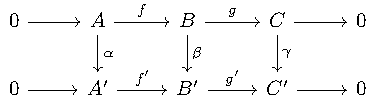
\includegraphics[scale=1.5]{images/fig_1.pdf}\\
                Figura \thefigcount. Diagrama del Lema de los cinco cortos.
                \stepcounter{figcount}
            \end{center}
        \end{minipage}
        \\

        un diagrama conmutativo de $R$-módulos y homomorfismos de $R$-módulos tal que cada fila es una secuencia exacta. Entonces:
        \begin{enumerate}[label = \textit{(\alph*)}]
            \item $\alpha,\gamma$ monomorfismos implica que $\beta$ es monomorfismo.
            \item $\alpha,\gamma$ epimorfismos implica que $\beta$ es epimorfismo.
            \item $\alpha,\gamma$ isomorfismos implica que $\beta$ es isomorfismo.
        \end{enumerate}
    \end{lema}

    \begin{proof}
        De \textit{(a)}: 
    \end{proof}



    \newpage

    \section{Ejercicios}

    \begin{obs}
        $R$ es un anillo.
    \end{obs}

    \begin{excer}
        Si $A$ es un grupo abeliano y $n>0$ es natural tal que $na=0$ para todo $a\in A$, entonces $A$ es un $\mathbb{Z}/\mathbb{Z}n$-módulo untario con la acción dada por:
        \begin{equation*}
            [k]a=ka,\quad\forall k\in\mathbb{Z}
        \end{equation*}
    \end{excer}

    \begin{proof}
        Primero, veremos que la acción está bien definida. En efecto, sean $k,l\in\mathbb{Z}$ tales que $[k]=[l]$, entonces $k-l\in\mathbb{Z}n$, es decir que existe $q\in\mathbb{Z}$ tal que:
        \begin{equation*}
            k-l=qn
        \end{equation*}
        Por tanto:
        \begin{equation*}
            \begin{split}
                [k]a&=ka\\
                &=(qn+l)a\\
                &=(qn)a+la\\
                &=0+la\\
                &=la\\
                &=[l]a\\
            \end{split}
        \end{equation*}
        por lo cual, la acción está bien definida. Veamos ahora que en efecto, $A$ es un $\mathbb{Z}/\mathbb{Z}n$-módulo:
        %TODO
        \begin{enumerate}[label = \textit{(\alph*)}]
            \item 
        \end{enumerate}
    \end{proof}

    \begin{excer}
        Sea $\cf{f}{A}{B}$ un homomorfismo de $R$-módulos.
        \begin{enumerate}[label = \textit{(\alph*)}]
            \item $f$ es monomorfismo si y sólo si para todo par de homomorfismos de $R$-módulos, $\cf{g,h}{D}{A}$ tales que $f\circ g=f\circ h$, tenemos que $g=h$.
            \item 
        \end{enumerate}
    \end{excer}

    \begin{proof}
        
    \end{proof}

    \begin{excer}
        Sea $I$ un ideal izquierdo de un anillo $R$ y sea $A$ un $R$-módulo.
        \begin{enumerate}[label = \textit{(\alph*)}]
            \item Si $S$ es un subconjunto no vacío de $A$, entonces
            \begin{equation*}
                IS=\left\{\sum_{ i=1}^n r_ia_i\Big|n\in\mathbb{N}^*;r_i\in I;a_i\in S \right\}
            \end{equation*}
            es un submódulo de $A$. Note que si $S=\left\{a \right\}$, entonces $IS=Ia=\left\{ra\Big|r\in I \right\}$.
            \item Si $I$ es un ideal por ambos lados, entonces $A/IA$ es un $R/I$ módulo con la acción de $R/I$ dada por:
            \begin{equation*}
                (r+I)(a+I)=ra+IA
            \end{equation*}
        \end{enumerate}
    \end{excer}

    \begin{proof}
        
    \end{proof}

    \begin{excer}
        Si $R$ tiene identidad, entonces todo $R$-módulo unitario cíclico es isomorfo a un $R$-módulo de la forma $R/J$, donde $J$ es un ideal izquierdo de $R$.
    \end{excer}

    \begin{proof}
        Sea $C$ el $R$-módulo unitario cíclico generado por $a$, esto es:
        \begin{equation*}
            C=\left\{ra\Big|r\in R \right\}
        \end{equation*}
        definimos el conjunto $J$ dado por:
        \begin{equation*}
            J=\left\{r\in R\Big|ra=0 \right\}
        \end{equation*}
        Afirmamos que $J$ es ideal izquierdo de $R$. En efecto, veamos que:
        \begin{enumerate}[label = \textit{(\arabic*)}]
            \item Sean $s,t\in J$, se tiene que:
            \begin{equation*}
                \begin{split}
                    (s-t)a&=sa-ta\\
                    &=0\\
                \end{split}
            \end{equation*}
            por ende, $s-t\in J$.
            \item Sea $s\in J$ y $r\in R$, se tiene que:
            \begin{equation*}
                \begin{split}
                    (rs)a&=r(sa)\\
                    &=r\cdot0\\
                    &=0\\
                \end{split}
            \end{equation*}
            por ende, $rs\in J$.
        \end{enumerate}
        por los dos incisos anteriores se sigue que $J$ es un ideal izquierdo de $R$. Por ejemplos anteriores se tiene que $R/J$ es un $R$-módulo. Considere la función $\cf{f}{C}{R/J}$ dado por:
        \begin{equation*}
            f(ra)=r+J,\quad\forall ra\in C
        \end{equation*}
        afirmamos que $f$ es un homomorfismo de $R$-módulos. En efecto:
        \begin{itemize}
            \item \textbf{$f$ es homomorfismo de $R$-módulos}. Sean $r_1a_1,r_2a_2\in C$. Se tiene:
            \begin{equation*}
                \begin{split}
                    f(r_1a_1+r_2a_2)&=r_1+r_2+J\\
                    &=(r_1+J)+(r_2+J)\\
                    &=f(r_1a_1)+f(r_2a_2)\\
                \end{split}
            \end{equation*}
            y, si $ra\in C$, entonces para $t\in R$ se tiene que:
            \begin{equation*}
                \begin{split}
                    f\left(t(ra) \right)&=f((tr)a)\\
                    &=tr+J\\
                    &=t(r+J)\\
                    &=tf(ra)\\
                \end{split}
            \end{equation*}
            \item \textbf{$f$ es monomorfismo}: Sea $ra\in C$. Veamos que:
            \begin{equation*}
                \begin{split}
                    f(ra)=J&\iff r+J=J\\
                    &\iff r\in J\\
                    &\iff ra=0\\
                \end{split}
            \end{equation*}
            por lo que, $\ker f=\left\{0 \right\}$.
            \item Para cada $r+J\in R/J$ existe $ar\in C$ tal que $f(ra)=r+J$.
        \end{itemize}
        por los tres incisos anteriores, se tiene que $f$ es isomorfismo de $R$-módulos.
    \end{proof}

    \begin{mydef}
        Si $R$ tiene identidad, entonces un $R$-módulo unitario $A$ no cero es \textbf{simple} si sus únicos submódulos son $0$ y $A$.
    \end{mydef}

    \begin{excer}
        Pruebe lo siguiente:
        \begin{enumerate}[label = \textit{(\arabic*)}]
            \item Todo $R$-módulo simple es cíclico.
            \item Si $A$ es simple, entonces todo $R$-módulo endomorfismo es la función cero o es un isomorifsmo.
        \end{enumerate}
    \end{excer}

    \begin{proof}
        De \textit{(1)}: Sea $A$ un $R$-módulo simple. Si $A$ no es el módulo $0$, entonces existe $c\in A$ no cero. Considere el $R$-módulo generado por $c$, digamos:
        \begin{equation*}
            C=\left\{rc+nc\Big|r\in R;n\in\mathbb{Z} \right\}
        \end{equation*}
        como $A$ es simple, debe suceder que $C=A$ ya que $c\neq0$ y $c\in C$. Por tanto, $A$ es cíclico.
        
        De \textit{(2)}: Sea $\cf{f}{A}{A}$ un $R$-módulo endomorfismo. Por un teorema anterior se tiene que $\ker f$ es un submódulo de $A$, el cual debe ser 0, lo cual implicaría que $f$ es isomorfismo, o es $A$, lo cual implicaría que $f$ es la función cero.
    \end{proof}

    \begin{excer}
        Pruebe que un $R$-módulo finitamente generado no necesariamente es un grupo abeliano finitamente generado.
    \end{excer}

    \begin{proof}
        Considere el grupo $(\mathbb{Q},+)$, se tiene que este grupo no es finitamente generado. En efecto, si lo fuese sería de la forma:
        \begin{equation*}
            \mathbb{Q}=\langle a_1,\dots,a_n \rangle
        \end{equation*}
        con $a_1,...,a_n\in\mathbb{Q}\setminus\left\{0\right\}$. Podemos asumir sin pérdida de generalidad que $a_i\geq 0$ para todo $i=1,...,n$. También, estos elementos son de la forma:
        \begin{equation*}
            a_i=\frac{p_i}{q_i},\quad\forall i=1,...,n
        \end{equation*}
        donde $p_i,q_i\in\mathbb{N}$ son primos relativos. Sea
        \begin{equation*}
            q=q_1\cdots q_n
        \end{equation*}
        Considere ahora el conjunto:
        \begin{equation*}
            A=\left\{qa\Big|a\in\langle a_1,\dots,a_n \rangle;a>0 \right\}
        \end{equation*}
        al ser todos los elementos de $\langle a_1,\dots,a_n \rangle$ sumas finitas de $a_i$, entonces se tiene que los elementos de $A$ son números naturales. Así que $A$ es un subconjunto de los naturales no vacío, en particular tiene primer elemento, digamos $p$. Se tiene que $\frac{p}{q}$ es el mínimo elemento positivo de $\langle a_1,\dots,a_n \rangle$. Ahora, sabemos que:
        \begin{equation*}
            \frac{p}{q+1}\in\mathbb{Q}
        \end{equation*}
        pero, $\frac{p}{q+1}\notin\langle a_1,\dots,a_n \rangle$, pues este elemento es menor que el mínimo elemento positivo de este conjunto\contradiction. Por ende, $\mathbb{Q}$ no es finitamente generado como grupo abeliano.

        Pero, $\mathbb{Q}$ es un $\mathbb{Q}$-módulo, el cual es finitamente generado por $1$ (se verifica rápidamente).
    \end{proof}

    \begin{excer}
        
    \end{excer}

    \begin{proof}
        
    \end{proof}

    \begin{excer}
        Sea $\cf{f}{A}{A}$ un homomorfismo de $R$-módulos tal que $f\circ f=f$, entonces:
        \begin{equation*}
            A=\ker f\oplus\im f
        \end{equation*}
    \end{excer}

    \begin{proof}
        Veamos primero que $A=\ker f+\im f$. Sea $a\in A$, si $a\notin\im f$, entonces veamos que:
        \begin{equation*}
            f(a)=f(f(a))\Rightarrow f(a-f(a))=0
        \end{equation*}
        por lo que, $a-f(a)\in\ker f$, luego $a\in\ker f+\im f$ (pues, $f(a)\in\im f$).

        Veamos ahora que es suma directa interna. En efecto, sea $a\in\ker f\cap\im f$, entonces existe $b\in A$ tal que:
        \begin{equation*}
            f(b)=a
        \end{equation*}
        como $a\in\ker f$ se sigue que $f(a)=0$. Observemos que:
        \begin{equation*}
            f(b)=f(f(b))=f(a)=0
        \end{equation*}
        por lo que, $b\in\ker f$, así que $a=f(b)=0$, esto es que $a=0$. Por tanto, se tiene que la suma es directa, esto es:
        \begin{equation*}
            A=\ker f\oplus\im f
        \end{equation*}
    \end{proof}

    \begin{excer}[Nombre]
        
    \end{excer}

    \begin{proof}
        
    \end{proof}

    \begin{excer}
        Haga lo siguiente:
        \begin{enumerate}[label = \textit{(\alph*)}]
            \item Si $A$ es un módulo sobre un anillo conmutativo $R$ y $a\in A$, entonces $\mathcal{O}_a=\left\{r\in R\Big|ra=0 \right\}$ es un ideal de $R$. Si $\mathcal{O}_a\neq0$, se dice que $a$ es un \textbf{elemento de torsión de $A$}.
            \item Si $R$ es un dominio entero, entonces el conjunto $T(A)$ de todos los elementos de torsión de $A$ es un submódulo de $A$ ($T(A)$ es llamado el \textbf{submódulo de torsión}).
            \item Muestre que el inciso anterior puede ser falso para un anillo conmutativo $R$ que no sea dominio entero.
        \end{enumerate}
        en lo que sigue, $R$ es un dominio entero.
        \begin{enumerate}[label = \textit{(\alph*)}]
            \setcounter{enumi}{3}
            \item Si $\cf{f}{A}{B}$ es un homomoifismo de $R$-módulos, entonces $f(T(A))\subseteq T(B)$; por ende, la reestricción $f_T$ de $f$ a $T(A)$ es un homomorfismo de $R$-módulos.
            \item Si $0\rightarrow A\overset{f}{\rightarrow}B\overset{g}{\rightarrow}C$ es una secuencia exacta de $R$-módulos, entonces también lo es $0\rightarrow T(A)\overset{f_T}{\rightarrow}T(B)\overset{g_T}{\rightarrow}T(C)$.
            \item 
        \end{enumerate}
    \end{excer}

    \newpage

    \chapter{Módulos Libres y Espacios Vectoriales}

    \section{Conceptos Fundamentales}

    No queda de otra más que asumir este resultado de categorías:

    \begin{theor}[\textbf{Hungerford, Theorem I.7.8}]
        Si $\mathcal{C}$ es una categoría concreta, $F$ y $F'$ son objetos en $C$ tales que $F$ es libre en el conjunto $X$ y $F'$ lo es en $X'$ siendo estos conjuntos tales que $\abs{X}=\abs{X'}$, entonces $F$ es equivalente a $F'$.
    \end{theor}

    En particular, la categoría de $R$-módulos unitarios es una categoría concreta, donde la equivalencia entre dos objetos de la categoría es un isomorfismo entre ambos $R$-módulos.

    \begin{theor}
        Sea $R$ un anillo conmutativo con identidad. Las siguientes condiciones son equivalentes en un $R$-módulo unitario $F$:
        \renewcommand{\theenumi}{\roman{enumi}}
        \begin{enumerate}
            \item $F$ tiene base no vacía.
            \item $F$ es la suma interna directa de una familia cíclica de $R$-módulos, cada uno de los cuales es isomorfo a $R$ como un $R$-módulo.
            \item $F$ es un $R$-módulo isomorfo a la suma directa de copias del $R$-módulo izquierdo $R$.
            \item Existe un conjunto no vacío $X$ y una función $\cf{i}{X}{F}$ con la siguiente propiedad: dado un $R$-módulo, $A$ y una función $\cf{f}{X}{A}$ existe un único homomorfismo de $R$-módulos $\cf{\overline{f}}{F}{A}$ tal que
            \begin{equation*}
                \overline{f}\circ i=f
            \end{equation*}
            En otras palabras, $F$ es un objeto libre en la categoría de $R$-módulos uniatrios.
        \end{enumerate}
    \end{theor}

    \begin{proof}
        $(i)\Rightarrow(iv)$: Sea $X$ una base no vacía de $F$ y sea $\cf{i}{X}{F}$ el mapeo inclusión. Sea $A$ un $R$-módulo y $\cf{f}{X}{A}$ una función.

        Si $u\in F$, entonces existen $n\in\mathbb{N}\cup\left\{0\right\}$, $r_i\in R$ y $x_i\in X$, para todo $i\in\left\{1,...,n\right\}$ tales que
        \begin{equation*}
            u=\sum_{ i=1}^n r_i x_i
        \end{equation*}
        Definimos la función $\cf{\overline{f}}{F}{A}$ dada por:
        \begin{equation*}
            \overline{f}(u)=\sum_{ i=1}^n r_if(x_i)
        \end{equation*}
        Esta función está bien definida, pues $F$ tiene como base a $X$ (por ende, todo elemento se representa de forma única como combinación lineal finita de elementos de $X$). Además,
        \begin{equation*}
            \begin{split}
                \overline{f}\circ i(x_i)&=\overline{f}(x_i)\\
                &=1_R\cdot f(x_i) \\
                &=f(x_i),\quad\forall x_i\in X \\
            \end{split}
        \end{equation*}
        por ende, $\overline{f}\circ i=f$.

        Veamos que es homomorfismo de $R$-módulos (no sé como se verifica eso, chécalo porfa Roque).

        Ahora, si $\cf{g}{F}{A}$ es otro homomorfismo de $R$-módulos tal que
        \begin{equation*}
            g\circ i=f
        \end{equation*}
        se tiene que
        \begin{equation*}
            \overline{f}\circ i=g\circ i\Rightarrow \overline{f}\big|_{X}=g\big|_{X}
        \end{equation*}
        Como $X$ genera $F$ y todo homomorfismo de $R$-módulos que vaya de $F$ en algún $R$-módulo, $B$ queda únicamente determinado por $X$, basta ver que $\overline{f}=g$ en $X$, lo cual sucede por la igualdad anterior. Por tanto, $\overline{f}$ es único.

        $(iv)\Rightarrow(iii)$: Asumiendo $(iv)$, sean $X\subseteq F$ no vacío y una función $\cf{i}{X}{F}$ que cumplan esta propiedad. Considere el $R$-módulo
        \begin{equation*}
            A=\sum_{ x\in X}R
        \end{equation*}
        (es decir, es la suma directa de $\abs{X}$-veces el $R$-módulo izquierdo $R$). Sea
        \begin{equation*}
            Y=\left\{\theta_x\Big| x\in X \right\}
        \end{equation*}
        donde
        \begin{equation*}
            \theta_x(y)=\left\{
                \begin{array}{lcr}
                    1_R & \textup{ si } & y=x\\
                    0_R & \textup{ si } & y\neq x\\
                \end{array}
            \right.,\quad\forall y\in Y
        \end{equation*}
        Como $X$ es no vacío, entonces $Y$ es no vacío. Por la parte $(iii)\Rightarrow(i)$, se sabe que $Y$ es una base del $R$-módulo unitario $A$. En particular, como $(iii)\Rightarrow(iv)$, se tiene que $A$ es un $R$-módulo libre en la categoría de $R$-módulos unitarios.
        
        En particular, $F$ y $A$ son $R$-módulos libres en la categoría de $R$-módulos unitarios y son tales que $\abs{X}=\abs{Y}$ (por la forma en que se construyó $Y$), luego por el Teorema anterior son equivalentes en esta categoría, es decir que existe un isomorfismo $\cf{f}{F}{A}$. Así que
        \begin{equation*}
            F\cong\sum_{ x\in X}R
        \end{equation*}
        lo que prueba el resultado.
    \end{proof}

    \section{Referencias}

    \begin{itemize}
        \item \textit{Algebra} de Thomas Hungerford, ed. Springer.
    \end{itemize}

\end{document}